\documentclass[12pt] {article}

%%% Preambuła %%%
\usepackage[T1]{fontenc}
\usepackage[polish]{babel}
\usepackage[utf8]{inputenc}
\usepackage{lmodern}
\usepackage{hyperref}
\usepackage{mathptmx}
\usepackage{float}
\usepackage{graphicx}
\usepackage{xcolor}
\selectlanguage{polish}
\usepackage{titlesec}

\definecolor{backgroundColor}{HTML}{3D3D3D}

%%% Strona tytułowa %%%
\title 
{	
	{
		\textbf{\textsf{\Huge\color{orange}DNS\color{white}ite}} \\ [0.1in]
		\normalfont\sffamily\LARGE\color{white}
		Aplikacja webowa do zarządzania serwerem DNS \\[0.1in]
		Dokumentacja użytkownika\\ [0.1in]
		\large 
		Inżynieria Oprogramowania \\
		Wydział Fizyki i Informatyki Stosowanej \\
		Informatyka Stosowana, 3 rok \\
	}
}

\author 
{
	\color{white}\normalfont\sffamily Arkadiusz Kasprzak \and 
	\color{white}\normalfont\sffamily Jarosław Cierpich \and 
	\color{white}\normalfont\sffamily Jakub Kowalski \and 
	\color{white}\normalfont\sffamily Konrad Pasik \and 
	\color{white}\normalfont\sffamily Krystian Molenda
}
\date{}


\titleformat{\section}
  {\normalfont\sffamily\Large\bfseries\color{orange}}
  {\thesection}{1em}{}

\titleformat{\subsection}
  {\normalfont\sffamily\large\bfseries\color{orange}}
  {\thesubsection}{1em}{}
	
\definecolor{ao}{rgb}{0.0, 0.0, 1.0}	
\definecolor{forestgreen(web)}{rgb}{0.13, 0.55, 0.13}

\begin{document}


%%% Strona tytułowa %%%
\pagecolor{backgroundColor}
\maketitle


\newpage
\pagecolor{white}

%%% Spis treści %%%
\tableofcontents

\newpage 

\section{Instalacja}
Aplikacja dostarczona została w postaci pliku \emph{fat JAR}, a zatem wszystkie biblioteki potrzebne do jej działania są już dołączone. Oprócz samej aplikacji do działania wymagane są:
\begin{itemize}
\item Java w wersji 8
\item Baza danych PostgreSQL 11
\item Aplikacja pgAdmin 4
\end{itemize}
W celu uruchomienia aplikacji należy \textbf{tutaj JAKUBIAN PODA CO}


\section{Pierwsze uruchomienie i konfiguracja}
Rozdział omawia proces pierwszego uruchomienia aplikacji oraz sposoby na zmianę konfiguracji aplikacji.

\subsection{Pierwsze uruchomienie}
Podczas pierwszego uruchomienia aplikacji wyświetlone zostanie następujące okno:
\begin{figure}[H]
\centering
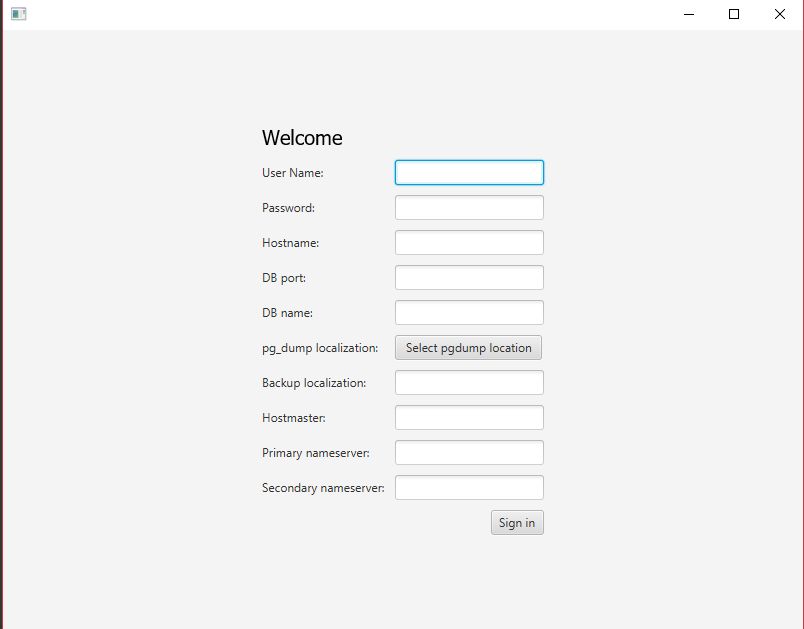
\includegraphics[scale=0.5]{res/1_konfiguracja}
\end{figure}
Służy ono do przeprowadzenia konfiguracji aplikacji - w szczególności wymaga od użytkownika szczegółów dotyczących bazy danych, z którą aplikacja ma się łączyć. Należy podać:
\begin{itemize}
\item Nazwę użytkownika posiadającego dostęp do bazy danych oraz prawa takie jak zapis czy odczyt z niej.
\item Hasło do bazy.
\item Nazwę hosta lub adres IP - np. \emph{localhost}.
\item Port, na którym dostępna jest baza.
\item Nazwę bazy danych, do której aplikacja ma się łączyć.
\end{itemize}
Ponadto interfejs zawiera dwa pola nieobowiązkowe:
\begin{itemize}
\item \emph{pg\_dump location} - ścieżka do narzędzie pg\_dump.exe, służącego do wykonywania kopii zapasowych danych z bazy PostgreSQL. Jest to oficjalne narzędzie dołączane przy instalacji programu pgAdmin.
\item \emph{Backup location} - ścieżka do katalogu, w którym przechowywane mają być kopie zapasowe danych z bazy
\end{itemize}
Ostatnie trzy pola są obowiązkowe:
\begin{itemize}
\item \emph{Hostmaster} - używane przy automatycznym tworzeniu rekordów SOA, gdy dodawana jest domena
\item \emph{Primary i Secondary nameserver} - domyślne serwery - podobnie jak wyżej, używane przy automatycznym tworzeniu rekordów SOA.
\end{itemize}
Po wprowadzeniu wszystkich koniecznych danych należy użyć przycisku \emph{Sign in}. Przeprowadzony zostanie test połączenia z bazą danych i jeśli zakończy się on pomyślnie, będzie można przejść do korzystania z właściwej części aplikacji.

\subsection{Zmiana konfiguracji}
Dostępne są dwa sposoby na ponowne przeprowadzenie procesu konfiguracji aplikacji:
\begin{itemize}
\item usunięcie pliku \textbf{dbconfig.yaml} - powoduje to ponowne uruchomienie opisanego powyżej graficznego interfejsu użytkownika przy następnym uruchomieniu aplikacji.
\item ręczna edycja pliku \textbf{dbconfig.yaml} - zapisane są w nim wszystkie parametry podane wcześniej za pomocą graficznego interfejsu użytkownika.
\end{itemize}

\section{Korzystanie z aplikacji}
Dostęp do aplikacji można uzyskać \textbf{za pomocą przeglądarki}. Po uruchomieniu należy wpisać w pasku adresu \url{http://localhost:8001/}. \newline
Kolejne podrozdziały zawierają opis podstawowych operacji, jakie można wykonać w aplikacji, takich jak logowanie, rejestracja, zmiana hasła czy edycja danych przechowywanych w bazie (rekordy, domeny).

\subsection{Logowanie i rejestracja}
Po uruchomieniu aplikacji w przeglądarce użytkownik powinien uzyskać dostęp do strony umożliwiającej logowanie, zawierającej przedstawiony poniżej formularz:
\begin{figure}[H]
\centering
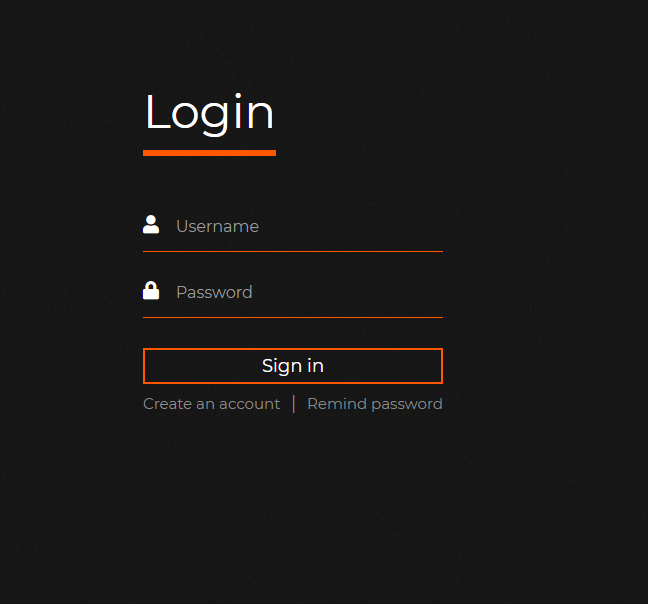
\includegraphics[scale=0.5]{res/2_logowanie}
\end{figure}
Umożliwia on wprowadzenie danych \textbf{logowania} (nazwa użytkownika i hasło ustalone przy rejestracji). W celu przeprowadzenie \textbf{rejestracji} należy wybrać opcję \emph{Create an account}. Wybranie jej przenosi do strony z następującym formularzem:
\begin{figure}[H]
\centering
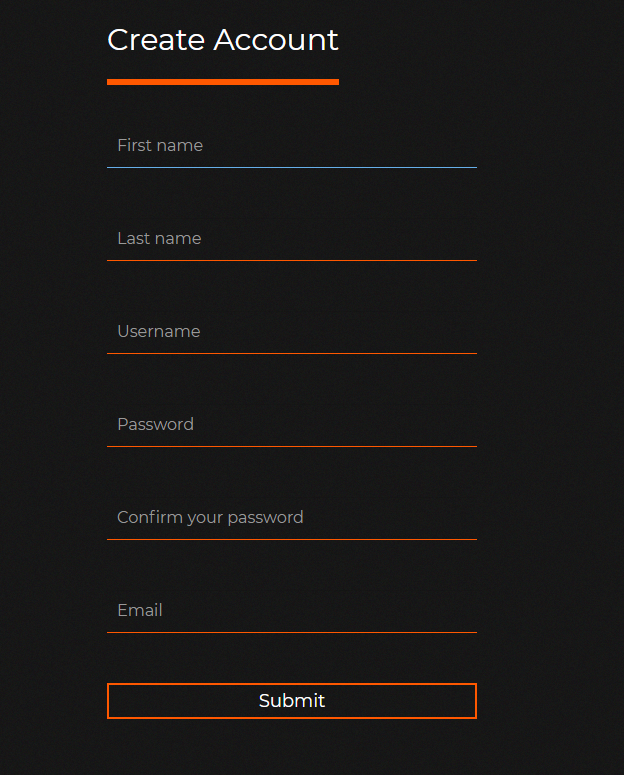
\includegraphics[scale=0.5]{res/3_rejestracja}
\end{figure}
Pierwszy utworzony użytkownik otrzymuje automatycznie prawa administratora i dostęp do aplikacji. Każdy następny musi zostać zatwierdzony przez zweryfikowane już konto (czyli konto mające dostęp do aplikacji). Do właściciela takiego konta wysyłana jest wiadomość e-mail z powiadomieniem.

\subsection{Rodzaje kont w aplikacji DNSite}
Aplikacja wyróżnia dwa rodzaje kont:
\begin{itemize}
\item konta zatwierdzone - konta mające pełny dostęp do aplikacji - przy ich pomocy można dokonać logowania. Pierwsze utworzone konto posiada taki status automatycznie.
\item konta niezatwierdzone - konta oczekujące na przyznanie dostępu do aplikacji - dostęp może zostać przyznany przez inne, już zatwierdzone konto
\end{itemize}


\subsection{Przypomnienie hasła}
W sytuacji, gdy użytkownik zapomni hasła do aplikacji, możliwe jest wygenerowanie nowego, tymczasowego. Użytkownik z poziomu panelu logowania powinien wybrać opcję \emph{Remind password}. Zostanie przeniesiony do panelu pokazanego poniżej:
\begin{figure}[H]
\centering
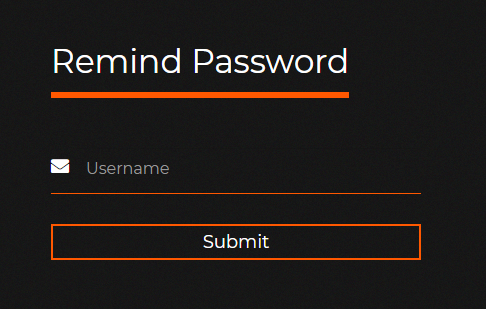
\includegraphics[scale = 1]{res/4_nowe_haslo}
\end{figure}
Po podaniu nazwy użytkownika i wybraniu opcji \emph{Submit}, do użytkownika zostanie wysłana wiadomość e-mail (na adres podany przy rejestracji). Będzie ona zawierać nowe, tymczasowe, wygenerowane losowo hasło, za pomocą którego użytkownik będzie mógł się zalogować do aplikacji. Przykładowa wiadomość została przedstawiona poniżej:
\begin{figure}[H]
\centering
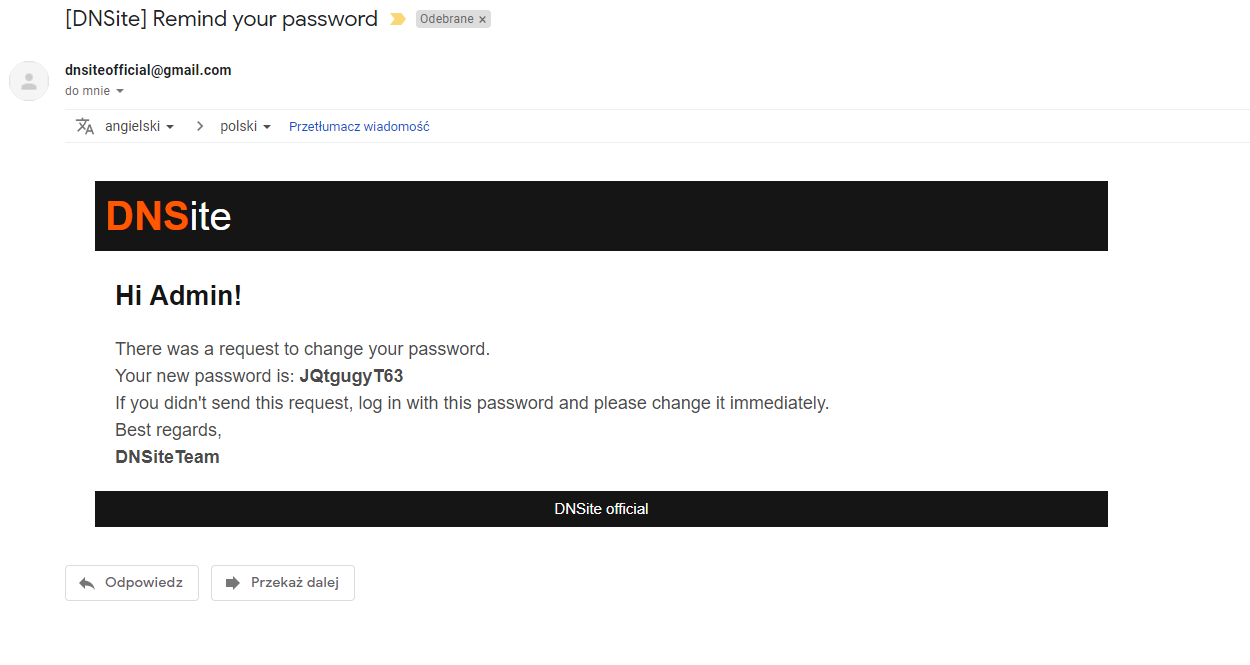
\includegraphics[width=\textwidth]{res/5_mail_haslo}
\end{figure}

\subsection{Strona główna aplikacji}
Po zalogowaniu się do aplikacji użytkownik uzyskuje dostęp do strony głównej:
\begin{figure}[H]
\centering
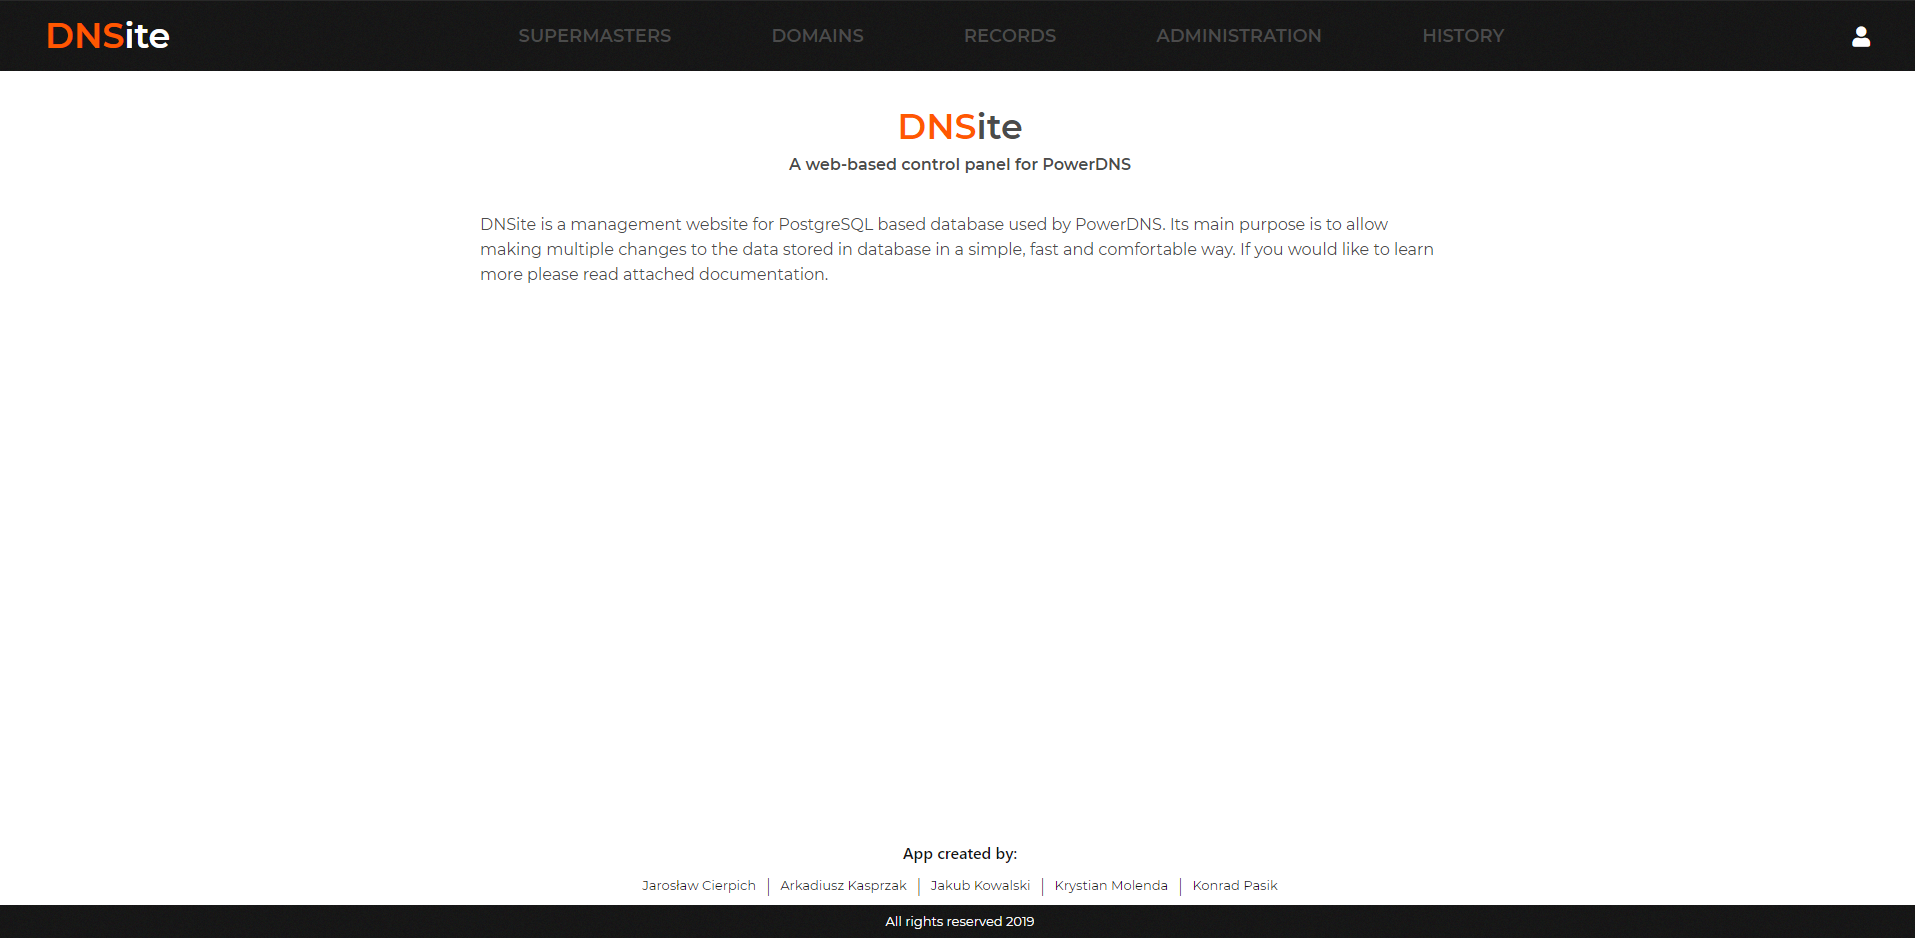
\includegraphics[width=\textwidth]{res/6_strona_glowna}
\end{figure}
W prawym górnym rogu znajduje się \emph{ikona użytkownika} - po jej wciśnięciu pojawia się menu zarządzania kontem:
\begin{figure}[H]
\centering
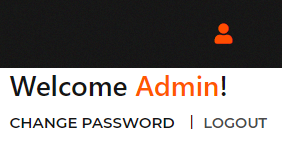
\includegraphics[scale = 1]{res/7_panel_uzytkownika}
\end{figure}
Umożliwia ono \textbf{wylogowanie} się z aplikacji oraz przeniesienie do panelu \textbf{zmiany hasła}. 

Panel nawigacyjny znajdujący się na stronie posiada odnośniki do widoków pozwalających użytkownikowi na przeprowadzenie wszelkich potrzebnych operacji na zasobach aplikacji i serwera DNS. Dostępne opcje:
\begin{itemize}
\item \textbf{Supermasters} - przeprowadzanie modyfikacji tabeli supermasters
\item \textbf{Domains} - przeprowadzanie operacji na domenach DNS
\item \textbf{Records} - przeprowadzanie operacji na rekordach DNS
\item \textbf{Administration} - strona umożliwiająca akceptowanie lub odrzucanie oczekujących na przyjęcie do aplikacji użytkowników
\item \textbf{History} - historia transakcji na bazie danych
\end{itemize}

Dolna część strony zawiera nazwiska autorów aplikacji - kliknięcie nazwiska danego autora przenosi użytkownika do konta w serwisie \textbf{Github}.

\subsection{Operacje na tabelach z danymi}
Rdzeniem funkcjonalności aplikacji \emph{DNSite} jest możliwość przeprowadzania operacji na bazie danych współdzielonej z serwerem \emph{PowerDNS}. W celu przeprowadzenia tychże operacji należy wybrać jedną z następujących opcji:
\begin{itemize}
\item Supermasters
\item Domains
\item Records
\end{itemize}
w panelu nawigacyjnym. W kilku kolejnych rozdziałach tego poradnika wykorzystany zostanie widok poświęcony rekordom DNS.

Praca na danych oparta jest na tabeli zbudowanej w ten sposób, by ułatwić wykonywanie wielu operacji w krótkim czasie. Komponent tabeli prezentuje się następująco:
\begin{figure}[H]
\centering
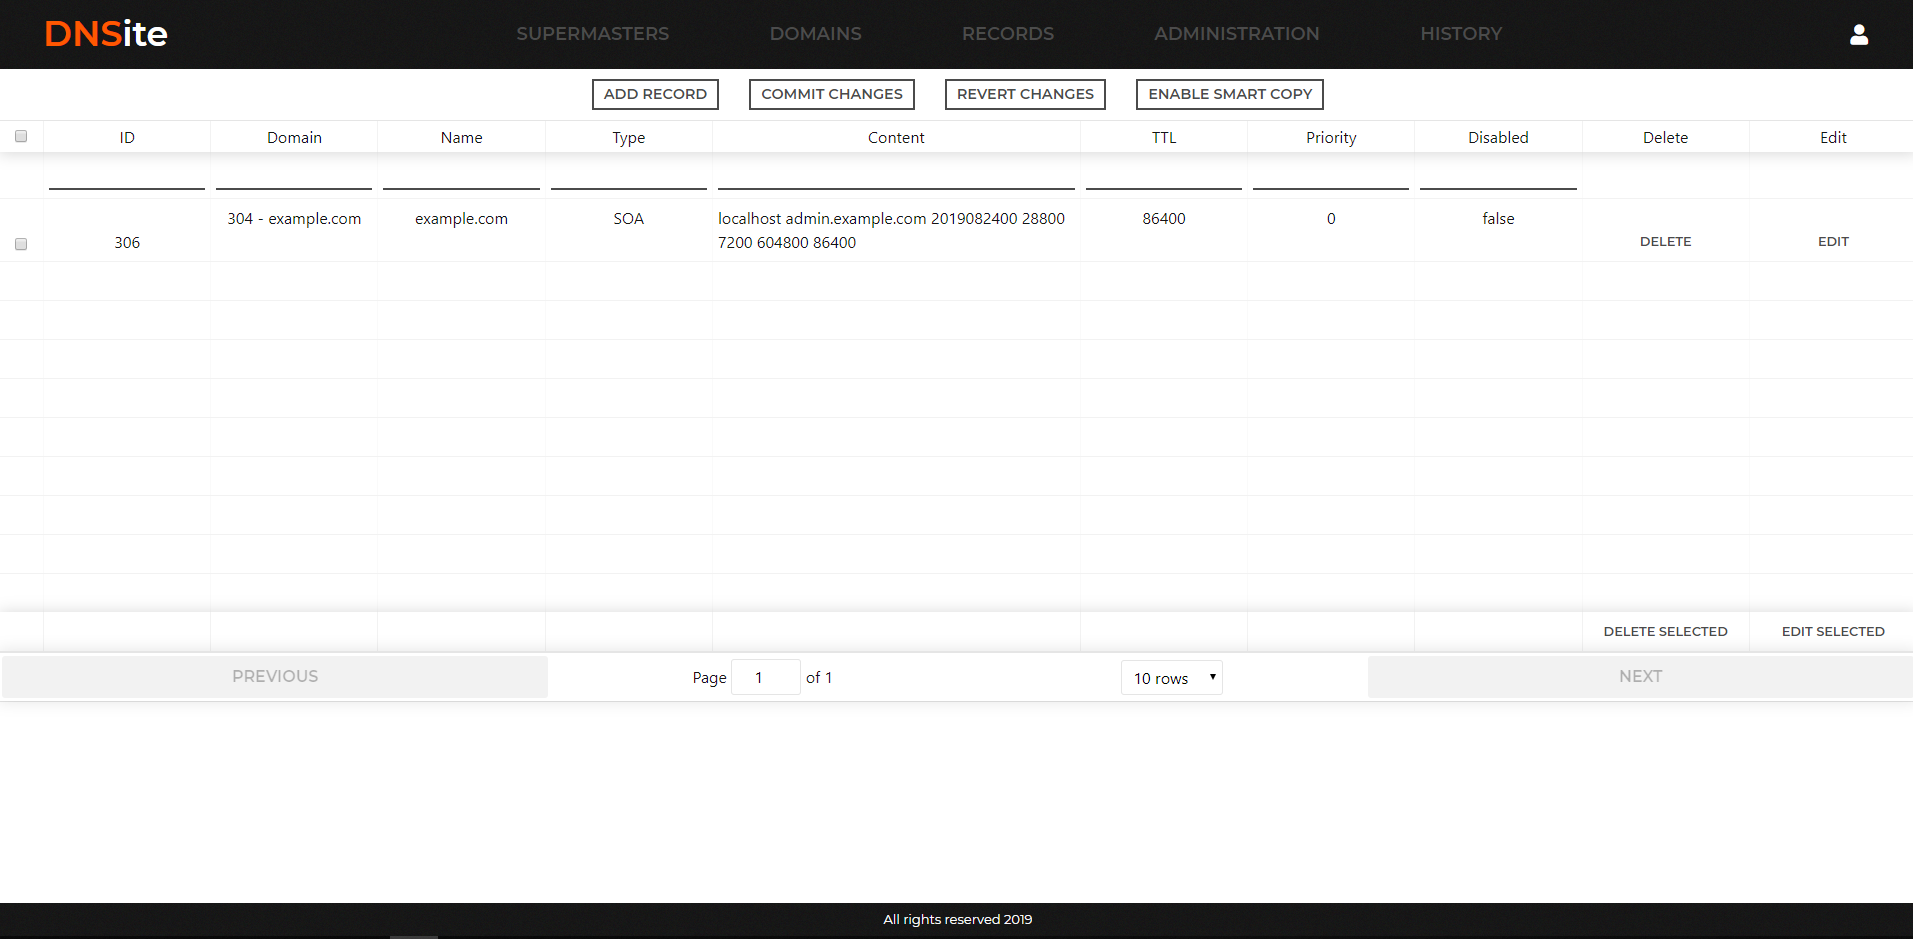
\includegraphics[width=\textwidth]{res/x_tabela}
\end{figure}

\subsection{Panel administratora}
Wybierając opcję \textbf{Administration} w panelu nawigacyjnym użytkownik zostaje przeniesiony do widoku panelu administracyjnego:
\begin{figure}[H]
\centering
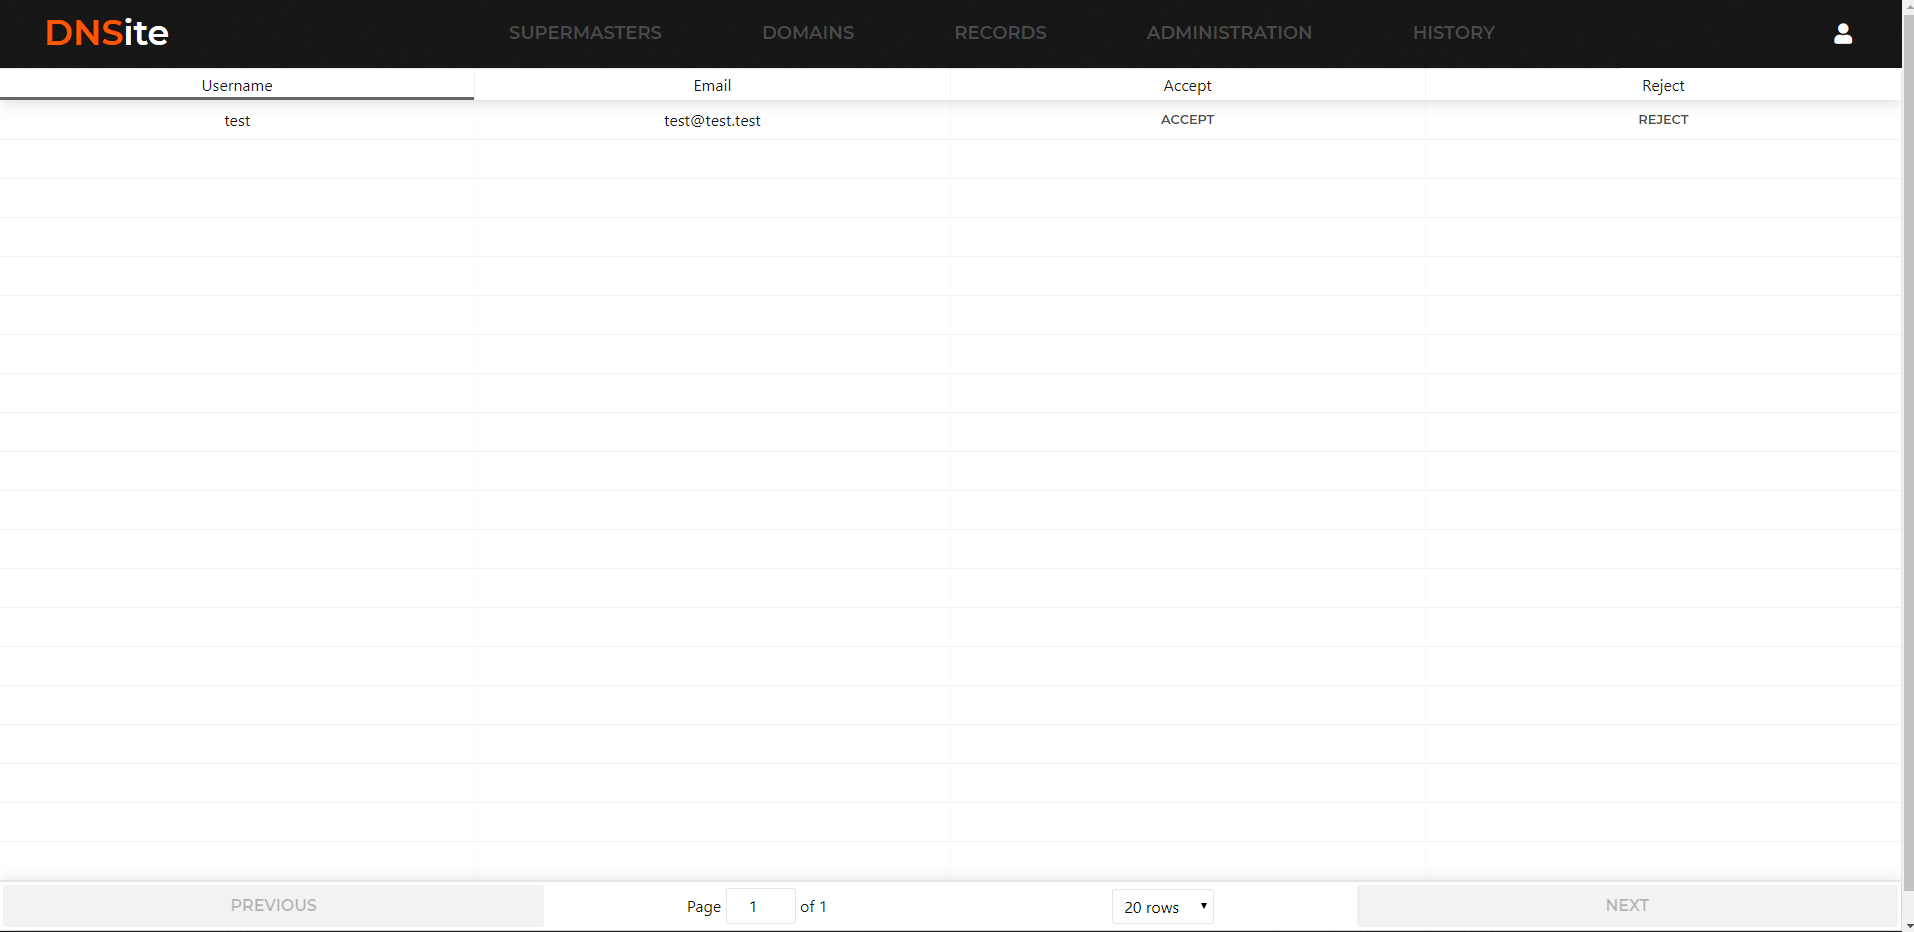
\includegraphics[width=\textwidth]{res/x_panel_administracyjny}
\end{figure}
Z poziomu tego panelu możliwe jest zatwierdzanie lub odrzucanie użytkowników oczekujących na przyznanie dostępu do aplikacji - można tego dokonać kolejno za pomocą przycisków \emph{Accept} oraz \emph{Reject}. 

\subsection{Panel historii}
Wybierając opcję \textbf{History} w panelu nawigacyjnym użytkownik zostaje przeniesiony do tabeli zawierającej historię transakcji przeprowadzanych na bazie danych:
\begin{figure}[H]
\centering
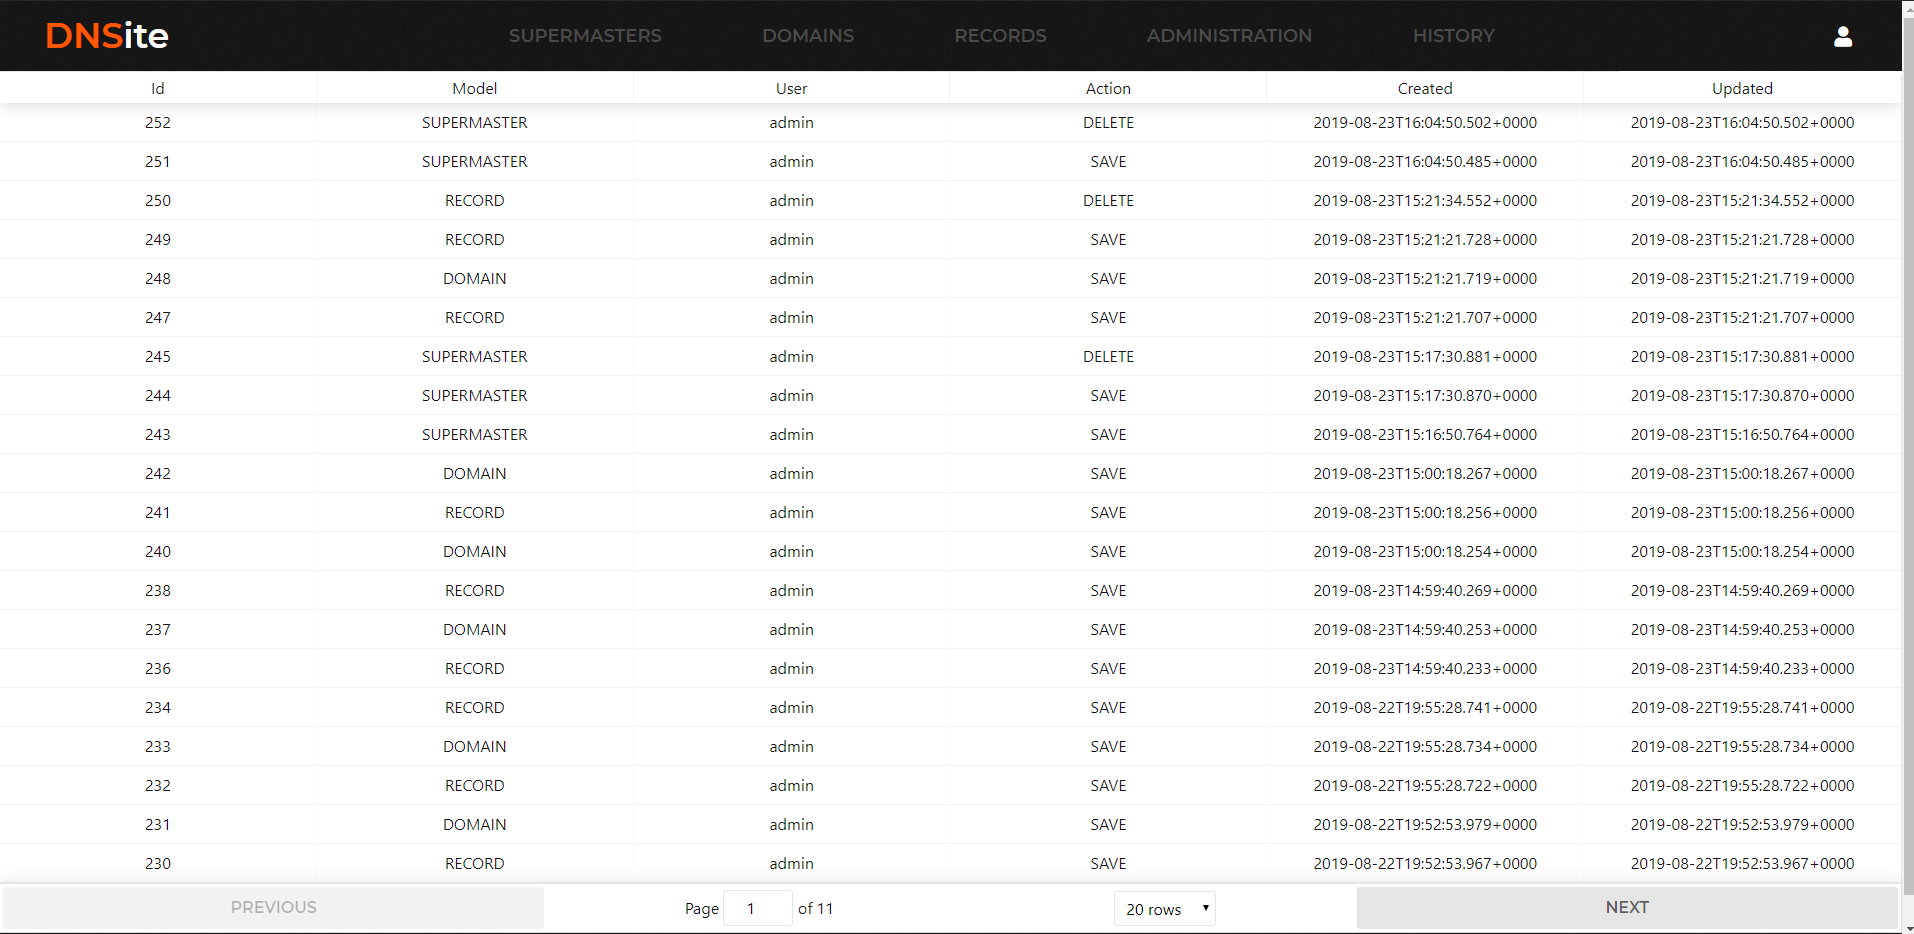
\includegraphics[width=\textwidth]{res/x_historia}
\end{figure}
Z tego poziomu użytkownik może przeglądać jakie zmiany w bazie zostały wprowadzone oraz kto je wprowadził. Kolumna \emph{Model} pokazuje, na jakim zasobie w bazie danych zmiana została przeprowadzona. 

\newpage
\section{Przewodnik użytkownika}



Interfejs graficzny służący do wprowadzania zmian w postaci tabelki:
\begin{figure}[H]
\centering
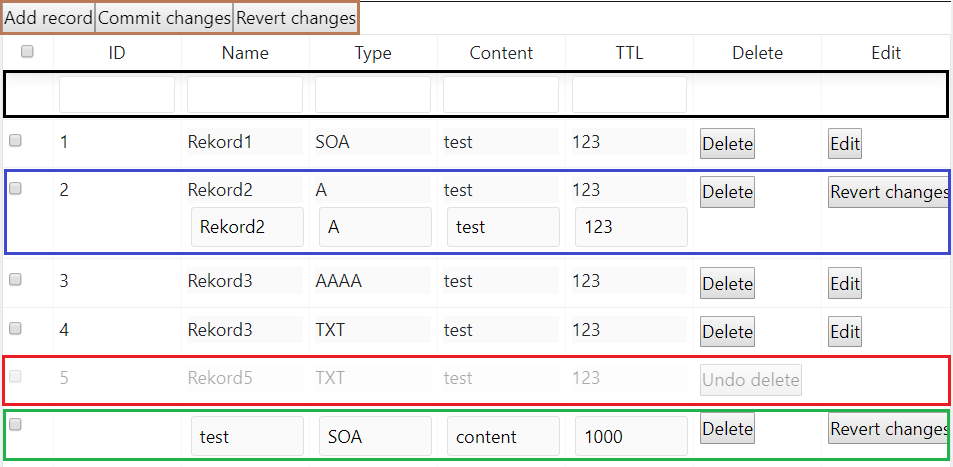
\includegraphics[width=\textwidth]{res/Tabelka}
\end{figure}


Możliwe operacje:
\begin{itemize}
\item \color{brown} Menu główne: 
\begin{itemize}
\item Dodanie nowego rekordu.
\item Zaaplikowanie wszystkim zmian i zaktualizowanie bazy danych
\item Powrót do stanu początkowego (wszystkie zmiany wprowadzone w trakcie sesji)
\end{itemize} \color{black}
\item \color{black} filtrowanie wyników \color{black}
\item \color{ao} edytowanie rekordu \color{black}
\item \color{red} usuwanie rekordu \color{black}
\item \color{forestgreen(web)} nowy wpis w tabelce - kontekst do dodania nowego rekordu \color{black}
\item Wprowadzenie zmian do wszystkich zaznaczonych i oznaczonych jako aktualnie edytowanych rekordów (niewidoczne na zrzucie ekranu)
\end{itemize}

Ważne informacje:
\begin{itemize}
\item Pola, gdzie mamy wybór spośród pewnej puli możliwości będą definiowane jako lista opcji (wybór jednej z możliwości)
\item Niektóre pola, np.: notified serial są tylko informacyjne i nie można ich zmieniać
\item Wszystkie widoki do edytowania są w formie tabelki, jedynym wyjątkiem są domeny, gdzie oprócz możliwości edytowania za pomocą listy jest również możliwość edytowania za pomocą formularza. 
\begin{figure}[H]
\centering
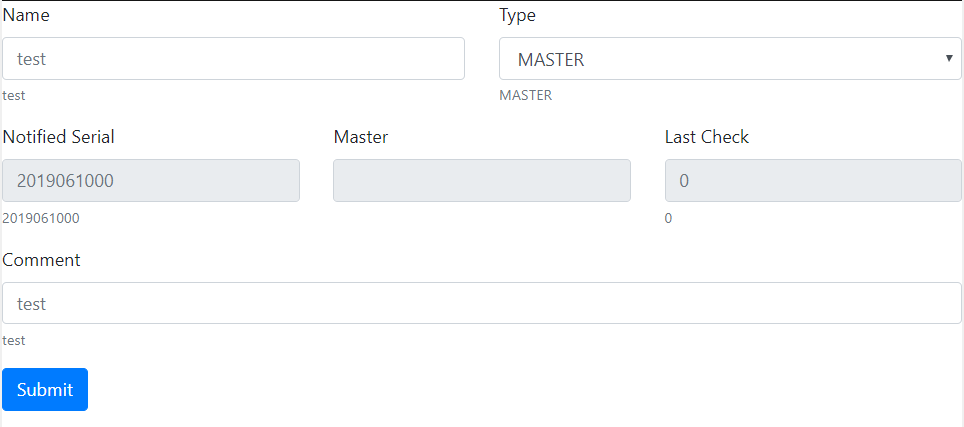
\includegraphics[width=\textwidth]{res/formularz}
\end{figure}
\end{itemize}

\end{document}